\documentclass[10pt]{article}

\usepackage[utf8]{inputenc}
\usepackage[T1]{fontenc}
\usepackage{lmodern}
\usepackage{amsmath,amssymb,amsthm}
\usepackage{array,booktabs}
\usepackage[table]{xcolor}
\usepackage{enumitem}
\usepackage{geometry}
\usepackage{hyperref}
\usepackage{algpseudocode}
\usepackage{float}
\usepackage[ruled, vlined, algoruled]{algorithm2e} % Options for styling
\usepackage{tikz}
\geometry{top=0.65in,bottom=0.65in,left=1.2in,right=1.2in}
\hypersetup{
  colorlinks=true,
  linkcolor=blue!60!black,
  urlcolor=cyan!50!black,
  linktoc=all
}
\setlist{nosep,leftmargin=*}
\renewcommand{\arraystretch}{1.2}
\newcolumntype{P}[1]{>{\raggedright\arraybackslash}p{#1}}

\theoremstyle{definition}
\newtheorem{definition}{Definition}[section]
\newtheorem{theorem}[definition]{Theorem}
\newtheorem{lemma}[definition]{Lemma}
\newtheorem{remark}[definition]{Remark}
\newtheorem{corollary}[definition]{Corollary}

\newcommand{\OPT}{\operatorname{OPT}}
\newcommand{\ALG}{\operatorname{ALG}}
\newcommand{\poly}{\operatorname{poly}}
\newcommand{\YES}{\textsc{Yes}}
\newcommand{\NO}{\textsc{No}}
\newcommand{\NP}{\mathsf{NP}}
\newcommand{\coNP}{\mathsf{coNP}}
\newcommand{\PTIME}{\mathsf{P}}
\newcommand{\NPC}{\mathsf{NP\text{-}complete}}

% Colours used to separate the three layers of approximation proofs.
\definecolor{algblue}{RGB}{0,82,155}
\definecolor{optred}{RGB}{180,45,45}
\definecolor{bridgepurple}{RGB}{105,55,145}

\title{CS4234: Optimization Algorithms}
\author{@Wxy2003-xy}
\date{}

\begin{document}

\maketitle
\tableofcontents
\newpage

\section*{Introduction and Prerequisites}
\subsection{Prerequisite map}

\begin{center}
\begin{tabular}{>{\bfseries}P{0.16\textwidth}P{0.34\textwidth}P{0.40\textwidth}}
\toprule
Source & Reusable idea & Role in CS4234 \\
\midrule
CS3230
& Asymptotic analysis, recurrences, and input encoding
& State running times in the true input length and distinguish polynomial
  from pseudo-polynomial algorithms. \\
CS3230
& Loop invariants, induction, exchange arguments, and optimal substructure
& Prove feasibility, optimality, approximation ratios, and termination. \\
CS3230
& Greedy algorithms, dynamic programming, graph algorithms, and randomization
& Supply exact subroutines and recurring algorithm-design patterns. \\
CS3230/CS4269
& Polynomial-time reductions and NP-completeness
& Explain why an exact polynomial-time algorithm may be unlikely and motivate
  relaxations, approximation, or restricted cases. \\
CS4269
& Propositional semantics, satisfiability, and formula encodings
& Turn combinatorial choices into Boolean or $0$--$1$ variables with explicit
  constraints. \\
\bottomrule
\end{tabular}
\end{center}

Topics such as compactness, Hilbert systems, first-order logic, and
computability remain useful background, but they are not part of this compact
optimization prerequisite.

\subsection{The optimization viewpoint}

An optimization problem separates the description of legal solutions from the
criterion used to rank them.

\begin{definition}[Optimization problem]
For an instance $I$, let $F(I)$ be its feasible set and let
$c_I\colon F(I)\to\mathbb{R}$ be its objective.  A minimization problem asks
for
\[
  \OPT(I)=\min_{x\in F(I)}c_I(x),
\]
while a maximization problem replaces $\min$ by $\max$.  A complete answer may
include both an optimal value and a witness $x^*$ attaining that value.
\end{definition}

The same problem often appears in three forms:
\begin{itemize}
  \item \textbf{decision:} is there a feasible solution of value at most $B$
        (minimization), or at least $B$ (maximization)?
  \item \textbf{search:} find any feasible solution, possibly satisfying a
        threshold;
  \item \textbf{optimization:} find the best feasible solution.
\end{itemize}
For an integer-valued objective known to lie in $[L,U]$, an optimization value
can often be recovered using $O(\log(U-L+1))$ calls to the decision problem.
This is a polynomial-time reduction when the endpoints have polynomial bit
length; the bound and encoding must be stated rather than silently assumed.

\paragraph{A standard model.}
Many problems can be written as
\[
  \min\{c^{\mathsf T}x:x\in F\},
\]
where $x$ records choices, $F$ records constraints, and $c$ records costs.
The domain of $x$ matters: $x\in\{0,1\}^n$ is discrete, whereas
$x\in[0,1]^n$ is a continuous relaxation.  Enlarging $F$ can make a problem
easier to solve, but may produce a solution that is not feasible for the
original problem.

\subsection{Asymptotics, input size, and cost models}

For eventually non-negative functions,
\begin{align*}
f\in O(g)
&\iff \exists C>0,\exists n_0,\forall n\ge n_0:\ f(n)\le Cg(n),\\
f\in \Omega(g)
&\iff \exists c>0,\exists n_0,\forall n\ge n_0:\ f(n)\ge cg(n),\\
f\in \Theta(g)
&\iff f\in O(g)\cap\Omega(g).
\end{align*}
Useful limit tests are
\[
\lim_{n\to\infty}\frac{f(n)}{g(n)}=0\Rightarrow f\in o(g),\qquad
0<\lim_{n\to\infty}\frac{f(n)}{g(n)}<\infty\Rightarrow f\in\Theta(g).
\]
The robust versions use $\limsup$ and $\liminf$ when the ratio oscillates.

\paragraph{Bit complexity.}
Running time is measured against the length of the encoded input, not merely
the numerical value of its parameters.  An integer $W$ requires
$\Theta(\log(W+1))$ bits in binary.  Consequently, a running time such as
$O(nW)$ is polynomial in the \emph{value} $W$ but can be exponential in its
bit length.  Such an algorithm is \textbf{pseudo-polynomial}.  This distinction
is central for knapsack-style dynamic programs and many weakly NP-hard
optimization problems.

\paragraph{Cost accounting.}
For every claimed bound, identify:
\begin{enumerate}
  \item the input-size parameters and their encodings;
  \item the number of iterations, states, or recursive calls;
  \item the cost of each operation or oracle call; and
  \item any hidden dependence on numerical precision.
\end{enumerate}
A recurrence such as $T(n)=aT(n/b)+f(n)$ is appropriate for recursive
decomposition.  Iterative optimization algorithms are often clearer as
\[
  \text{preprocessing cost}
  + (\text{number of iterations})(\text{cost per iteration}).
\]

\subsection{Proof obligations for algorithms}

The loop-invariant template from CS3230 remains the default proof pattern:
\emph{initialization}, \emph{maintenance}, and \emph{termination}.  For a
recursive algorithm, replace the invariant by induction on the instance size.
For optimization, separate the claims that are easy to accidentally conflate.

\begin{enumerate}
  \item \textbf{Feasibility:} the returned solution lies in $F(I)$.
  \item \textbf{Value guarantee:} its objective satisfies the promised bound.
  \item \textbf{Optimality or approximation:} compare it with every feasible
        solution, a lower/upper bound, or an optimal witness.
  \item \textbf{Termination and complexity:} the procedure finishes within the
        claimed resources under the stated computational model.
\end{enumerate}

For a non-negative objective and an $\alpha$-approximation with $\alpha\ge1$,
the usual conventions are
\[
\begin{array}{ll}
\text{minimization:} & \OPT(I)\le\ALG(I)\le\alpha\OPT(I),\\[2pt]
\text{maximization:} & \OPT(I)/\alpha\le\ALG(I)\le\OPT(I).
\end{array}
\]
Feasibility gives one side of each inequality; the real proof is the other
side.  A common strategy is to compare the algorithm against a certificate
bound $L(I)\le\OPT(I)$ for minimization or $U(I)\ge\OPT(I)$ for maximization.

\paragraph{Reusable proof patterns.}
\begin{itemize}
  \item \textbf{Exchange argument:} transform an optimum so that it agrees
        with the greedy choice without worsening its value.
  \item \textbf{Optimal substructure:} after fixing a decision, the remainder
        is an optimal solution to a well-defined subproblem.
  \item \textbf{Charging argument:} charge the cost of the computed solution
        to parts of an optimum, with bounded charge per part.
  \item \textbf{Relaxation bound:} compare an integral solution with the value
        of a relaxation whose feasible region contains all integral solutions.
\end{itemize}

\subsection{Algorithm-design tools retained from CS3230}

\paragraph{Dynamic programming.}
A DP proof should state the subproblem, recurrence, base cases, evaluation
order, and recovery of a witness.  If $D[s]$ denotes the best value for state
$s$, the key equality is justified by partitioning all feasible solutions by
their last decision:
\[
  D[s]=\operatorname*{opt}_{a\in A(s)}
       \{\operatorname{cost}(s,a)+D[\operatorname{next}(s,a)]\}.
\]
The running time is the number of reachable states times the transition cost.
State coordinates that range up to a numeric value such as a capacity $W$ are
where pseudo-polynomial behaviour usually enters.

\paragraph{Greedy algorithms.}
A locally best choice is not a proof.  Correctness normally requires an
exchange argument, a stays-ahead invariant, or a structural property such as
a cut property.  When no such proof exists, the same greedy rule may still be
useful as a heuristic or approximation algorithm, but its guarantee must be
analysed separately.

\paragraph{Graph subroutines.}
Shortest paths, minimum spanning trees, maximum flow, matching, and
connectivity recur as exact subroutines and as sources of relaxations.  Always
record their preconditions: for example, Dijkstra's algorithm requires
non-negative edge weights, whereas Bellman--Ford permits negative edges but
must detect reachable negative cycles.

\subsection{Probability toolkit for randomized optimization}

Let $X_1,\ldots,X_n$ be random variables and let
$X=\sum_i X_i$.  The most reusable facts from CS3230 are
\begin{align*}
\mathbb{E}[X]&=\sum_i\mathbb{E}[X_i]
&&\text{(no independence required)},\\
\Pr\!\left[\bigcup_i A_i\right]&\le\sum_i\Pr[A_i]
&&\text{(union bound)},\\
\Pr[X\ge t]&\le\frac{\mathbb{E}[X]}{t}
&&\text{for $X\ge0$ (Markov)}.
\end{align*}
Indicator variables $X_i=\mathbf{1}[A_i]$ turn counting questions into
expectations because $\mathbb{E}[X_i]=\Pr[A_i]$.

For independent Bernoulli variables with $\mu=\mathbb{E}[X]$ and
$0<\delta<1$, useful Chernoff forms are
\[
  \Pr[X\le(1-\delta)\mu]\le e^{-\delta^2\mu/2},\qquad
  \Pr[X\ge(1+\delta)\mu]\le e^{-\delta^2\mu/(2+\delta)}.
\]
These concentration inequalities require stronger assumptions than linearity
of expectation; independence must be checked rather than silently assumed.

If one independent run fails with probability at most $q<1$, then $t$ runs
all fail with probability at most $q^t$.  This is the amplification principle
seen in Freivalds' algorithm.  In optimization it also supports randomized
rounding: solve a fractional relaxation, interpret fractional coordinates as
selection probabilities, and prove objective and feasibility bounds using
expectation plus concentration.

\subsection{Logic and constraint modelling from CS4269}

A propositional formula has \emph{syntax}; a valuation gives it
\emph{semantics}.  For a valuation $v$,
\begin{itemize}
  \item $v\models\phi$ means that $v$ satisfies $\phi$;
  \item $\phi$ is satisfiable if some $v$ satisfies it;
  \item $\phi$ is valid if every $v$ satisfies it;
  \item $\Gamma\models\phi$ means every model of $\Gamma$ is a model of
        $\phi$; and
  \item $\phi\equiv\psi$ means the two formulas have the same models.
\end{itemize}
The distinction between satisfiability and validity matters: a feasible
solution corresponds to \emph{one} satisfying assignment, not to a formula
that is true under all assignments.

\paragraph{Constraint-encoding recipe.}
The graph-colouring, Hamiltonian-path, clique, exact-cover, and scheduling
encodings in CS4269 share one pattern:
\begin{enumerate}
  \item introduce a variable for each atomic choice;
  \item write separate constraints for existence, uniqueness, compatibility,
        and global requirements;
  \item conjoin the constraints into one formula;
  \item prove a two-way correspondence between models and feasible solutions;
  \item prove that the encoding has polynomial size and is computable in
        polynomial time.
\end{enumerate}
For variables $p_1,\ldots,p_k$, ``exactly one'' is
\[
  \left(\bigvee_{i=1}^k p_i\right)
  \land
  \left(\bigwedge_{1\le i<j\le k}(\neg p_i\lor\neg p_j)\right).
\]
The first part gives existence; the pairwise clauses give uniqueness.

\subsection{From Boolean constraints to binary optimization}

Set $x_i=1$ when proposition $p_i$ is true and $x_i=0$ otherwise.  Common
logical constraints then become linear inequalities:

\begin{center}
\begin{tabular}{P{0.36\textwidth}P{0.43\textwidth}}
\toprule
Boolean constraint & $0$--$1$ linear form \\
\midrule
$p_1\lor\cdots\lor p_k$
  & $x_1+\cdots+x_k\ge1$ \\
$p\rightarrow q$
  & $x_p\le x_q$ \\
exactly one of $p_1,\ldots,p_k$
  & $x_1+\cdots+x_k=1$ \\
$z\leftrightarrow(p\land q)$
  & $z\le x_p$, $z\le x_q$, and $z\ge x_p+x_q-1$ \\
clause $\ell_1\lor\cdots\lor\ell_k$
  & $\sum_{\ell_i=p_j}x_j+\sum_{\ell_i=\neg p_j}(1-x_j)\ge1$ \\
\bottomrule
\end{tabular}
\end{center}

\paragraph{Example: minimum vertex cover.}
For a graph $G=(V,E)$, let $x_v$ indicate whether vertex $v$ is selected:
\[
  \min\sum_{v\in V}x_v
  \quad\text{subject to}\quad
  x_u+x_v\ge1\quad\forall\{u,v\}\in E,
  \qquad x_v\in\{0,1\}.
\]
Each edge constraint is the clause $p_u\lor p_v$.  Replacing
$x_v\in\{0,1\}$ by $0\le x_v\le1$ gives a linear relaxation.  Its feasible
region is larger, so for this minimization problem its optimum is a lower
bound on the integral optimum.

\subsection{Complexity classes and reductions}

\begin{definition}[Core classes]
$\PTIME$ is the class of decision problems solvable in polynomial time.
$\NP$ is the class whose \YES{} instances have polynomial-size certificates
verifiable in polynomial time.  A problem $B$ is NP-hard if every problem in
$\NP$ polynomial-time reduces to $B$; it is NP-complete if, in addition,
$B\in\NP$.
\end{definition}

A polynomial-time many-one reduction $A\le_p B$ is a polynomial-time
computable map $f$ such that
\[
  x\in A\iff f(x)\in B.
\]
The direction has an operational meaning: an algorithm for $B$ would yield an
algorithm for $A$.  To prove that $B$ is hard, reduce a known hard problem
\emph{to} $B$, not the other way around.

Every reduction proof has three obligations:
\begin{enumerate}
  \item \textbf{construction:} define $f(x)$ completely;
  \item \textbf{correctness:} prove both directions of
        $x\in A\iff f(x)\in B$; and
  \item \textbf{complexity:} prove that $f$ runs in polynomial time and its
        output has polynomial encoded size.
\end{enumerate}
The SAT encodings from CS4269 are reductions when they satisfy exactly these
obligations.  Cook--Levin supplies the central starting point: SAT is
NP-complete.

\paragraph{Decision versus optimization hardness.}
NP-completeness formally applies to decision problems.  To discuss an
optimization problem, define its threshold version.  For example, the
decision version of minimum vertex cover asks whether a cover of size at most
$k$ exists.  If an exact optimizer ran in polynomial time, evaluating whether
its returned value is at most $k$ would solve this decision problem in
polynomial time.  Thus NP-hardness of the threshold problem implies NP-hardness
of exact optimization.

\subsection{A checklist for the rest of CS4234}

For each new problem or algorithm, record the following before doing algebra:
\begin{enumerate}
  \item What is the instance, and what is its encoded length?
  \item What are the variables, feasible solutions, and objective direction?
  \item Is the task decision, search, or optimization?
  \item What invariant, exchange, induction, charging, or relaxation argument
        proves the guarantee?
  \item Is the guarantee exact, approximate, expected, or with high
        probability?
  \item Does the runtime depend polynomially on the bit length, or only on a
        numerical value?
  \item For a reduction, is the direction correct, is the equivalence proved
        both ways, and is the construction polynomial in encoded size?
\end{enumerate}

\bigskip


\section{Formulae and Theorems}
\subsection{Basic Probability Identities}
\[
\Pr(A\cup B)\le \Pr(A)+\Pr(B)\quad\text{(\textbf{Union bound})}
\]
\[
\Pr(A\cup B)=\Pr(A)+\Pr(B)-\Pr(A\cap B)\quad\text{(Inclusion--Exclusion, 2 terms)}
\]
\[
\Pr(A\mid B)=\frac{\Pr(A\cap B)}{\Pr(B)},\quad A\perp B\iff \Pr(A\cap B)=\Pr(A)\Pr(B)
\]
\[
\text{Law of Total Probability: }\ \Pr(A)=\sum_i \Pr(A\mid E_i)\Pr(E_i),\ \{E_i\}\text{ partition}
\]
\[
\text{Bayes: }\ \Pr(H\mid D)=\frac{\Pr(D\mid H)\Pr(H)}{\Pr(D)}
\]

\subsection{Indicator Trick \& Linearity}
For indicator $I_E=\mathbf{1}\{E\}$: $\ \mathbb{E}[I_E]=\Pr(E)$.
For a sum $X=\sum_{i=1}^n I_i$ (\emph{counting something}):
\[
\mathbb{E}[X]=\sum_{i=1}^n \Pr(I_i=1)\quad\text{(no independence needed)}
\]
If $I_i$ are pairwise independent: 
\[
\mathrm{Var}(X)=\sum_{i=1}^n \mathrm{Var}(I_i)=\sum_i p_i(1-p_i)
\]

\subsection{Expectation/Variance Identities}
\[
\mathbb{E}[aX+b]=a\,\mathbb{E}[X]+b\quad\text{(Linearity)}
\]
\[
\mathbb{E}[X]=\mathbb{E}\big[\ \mathbb{E}[X\mid Y]\ \big]\quad\text{(Law of total expectation)}
\]
\[
\mathrm{Var}(X)=\mathbb{E}[X^2]-\mathbb{E}[X]^2
\]
\[
\mathrm{Var}(X)=\mathbb{E}\!\left[\mathrm{Var}(X\mid Y)\right]+\mathrm{Var}\!\left(\mathbb{E}[X\mid Y]\right)\quad\text{(Law of total variance)}
\]
\[
\text{Tail-sum (nonneg. integer $X$): }\ \mathbb{E}[X]=\sum_{t\ge1}\Pr[X\ge t]
\]

\subsection{Inequalities (Concentration)}
\[
\Pr(X\ge a)\le \frac{\mathbb{E}[X]}{a}\quad\text{(\textbf{Markov})}
\]
\[
\Pr(|X-\mu|\ge t)\le \frac{\mathrm{Var}(X)}{t^2}\quad\text{(\textbf{Chebyshev})}
\]

\noindent\textbf{Chernoff/Hoeffding for sums of bounded/0--1 r.v.'s.} Let $X=\sum_{i=1}^n X_i$, $X_i\in[0,1]$ independent, $\mu=\mathbb{E}[X]$.
\[
\Pr\!\left[X\ge (1+\delta)\mu\right]\le \exp\!\left(-\frac{\mu\,\delta^2}{2+\delta}\right)\quad(\delta>0)
\]
\[
\Pr\!\left[X\le (1-\delta)\mu\right]\le \exp\!\left(-\frac{\mu\,\delta^2}{2}\right)\quad(0<\delta<1)
\]
\[
\Pr(|X-\mu|\ge t)\le 2\exp\!\left(-\frac{2t^2}{n}\right)\quad\text{(Hoeffding, if $X_i\in[0,1]$)}
\]
\emph{Handy simplification for $0<\delta\le1$: } $\Pr(|X-\mu|\ge \delta\mu)\le 2\exp(-\mu\delta^2/3)$.
\subsection{Common Inequalities for Mathematical Proofs}
Many mathematical arguments rely on a small set of fundamental inequalities.
Below is a unified chain collecting the most frequently used algebraic,
geometric, convexity, and analytic inequalities.  Each tool is stated in a form
that is easy to substitute directly into proofs.
\paragraph{Master Chain of Useful Inequalities.}

\subsubsection*{(1) Basic Algebraic Inequalities}
\[
a \le b \Rightarrow a+c \le b+c,
\qquad
a \le b,\ c \ge 0 \Rightarrow ac \le bc.
\]
\[
(a-b)^2 \ge 0
\;\Rightarrow\;
2ab \le a^2 + b^2
\;\Rightarrow\;
|ab| \le \frac{a^2 + b^2}{2}.
\]

\subsubsection*{(2) AM--GM--HM Hierarchy}
For all \(a,b>0\),
\[
\frac{a+b}{2} \ge \sqrt{ab} \ge \frac{2}{\tfrac{1}{a}+\tfrac{1}{b}}.
\]

\subsubsection*{(3) Cauchy--Schwarz Inequality}
\[
\left(\sum_{i=1}^n a_i b_i\right)^2
\le
\left(\sum_{i=1}^n a_i^2\right)
\left(\sum_{i=1}^n b_i^2\right).
\]

\subsubsection*{(4) Triangle Inequality}
\[
|x+y|\le |x|+|y|,
\qquad
\|u+v\| \le \|u\| + \|v\|.
\]

\subsubsection*{(5) Jensen's Inequality (Convex Functions)}
If \(f\) is convex and \(\lambda_i \ge 0\), \(\sum \lambda_i = 1\),
\[
f\!\left(\sum_{i=1}^n \lambda_i x_i\right)
\le
\sum_{i=1}^n \lambda_i f(x_i).
\]

\subsubsection*{(6) Bernoulli's Inequality}
For \(x \ge -1\),
\[
(1+x)^r \ge 1 + rx
\qquad (r \ge 1 \text{ or } r \le 0).
\]

\subsubsection*{(7) Weighted AM--GM}
If \(a_i > 0\), \(\alpha_i \ge 0\), \(\sum\alpha_i = 1\),
\[
a_1^{\alpha_1} a_2^{\alpha_2}\cdots a_n^{\alpha_n}
\le
\alpha_1 a_1 + \alpha_2 a_2 + \cdots + \alpha_n a_n.
\]

\subsubsection*{(8) Young's Inequality}
For \(p,q>1\), \(\tfrac{1}{p}+\tfrac{1}{q}=1\),
\[
ab \le \frac{a^p}{p} + \frac{b^q}{q}.
\]

\subsubsection*{(9) Hölder's Inequality}
\[
\|fg\|_1 \le \|f\|_p \|g\|_q,
\qquad
p,q>1,\quad \frac{1}{p}+\frac{1}{q}=1.
\]

\subsubsection*{(10) Logarithmic Inequalities}
\[
\ln(1+x)\le x,\qquad
1+x \le e^x,\qquad
\ln x \le x-1.
\]

\subsubsection*{(11) Exponential Bounds}
\[
1+x \le e^x \le 1 + x + \frac{x^2}{2}e^{|x|}.
\]

\subsubsection*{(12) Chebyshev's Sum Inequality}
For similarly sorted sequences,
\[
\frac{1}{n}\sum_{i=1}^n a_i b_i
\ge
\left(\frac{1}{n}\sum_{i=1}^n a_i\right)
\left(\frac{1}{n}\sum_{i=1}^n b_i\right).
\]

\subsubsection*{(13) Rearrangement Inequality}
For sorted \(a_1 \le \cdots \le a_n\),
\[
\sum_{i=1}^n a_i b_i
\le
\sum_{i=1}^n a_i b_{\sigma(i)}
\le
\sum_{i=1}^n a_i b_i^{\downarrow}.
\]

\subsubsection*{(14) Markov and Chebyshev Bounds}
\[
\Pr[X\ge a] \le \frac{\mathbb{E}[X]}{a},
\qquad
\Pr\big(|X-\mu|\ge t\big)\le \frac{\operatorname{Var}(X)}{t^2}.
\]

\subsubsection*{(15) Jensen + Logarithm = AM--GM}
\[
\ln\!\left(\frac{a_1+\cdots+a_n}{n}\right)
\ge
\frac{1}{n}\sum_{i=1}^n \ln a_i.
\]

\paragraph{Notes.}
\begin{itemize}
    \item Inequalities (1)--(4) handle almost all algebraic manipulations in proofs.
    \item (5)--(8) come from convexity and are widely used in optimization and analysis.
    \item (9)--(13) generalize inner-product arguments and are essential in analysis.
    \item (14)--(15) appear frequently in algorithm analysis and probability arguments.
\end{itemize}
\subsection{Common Taylor Series Expansions}

In this subsection we list the most frequently used Taylor (and Maclaurin)
series expansions.  Unless stated otherwise, all expansions are Maclaurin
series (expansion at \(x=0\)) and hold for sufficiently small \(|x|\).

\subsubsection*{(1) Exponential Function}
\[
e^x
    = 1 + x + \frac{x^2}{2!} + \frac{x^3}{3!} + \cdots
    = \sum_{n=0}^\infty \frac{x^n}{n!}.
\]
Useful bounds:
\[
1+x \le e^x \le 1 + x + \frac{x^2}{2}e^{|x|}.
\]

\subsubsection*{(2) Natural Logarithm}
For \(|x|<1\),
\[
\ln(1+x)
    = x - \frac{x^2}{2} + \frac{x^3}{3} - \frac{x^4}{4} + \cdots
    = \sum_{n=1}^\infty (-1)^{n+1}\frac{x^n}{n}.
\]
Special asymptotic form:
\[
\ln(1+x) = x - \frac{x^2}{2} + O(x^3).
\]

\subsubsection*{(3) Geometric Series}
For \(|x|<1\),
\[
\frac{1}{1-x}
    = 1 + x + x^2 + x^3 + \cdots.
\]

\subsubsection*{(4) Binomial Series}
For any real \(\alpha\), and \(|x|<1\),
\[
(1+x)^\alpha
    = \sum_{n=0}^{\infty}
      {\alpha \choose n} x^n
    = 1 + \alpha x + \frac{\alpha(\alpha-1)}{2}x^2
        + \frac{\alpha(\alpha-1)(\alpha-2)}{6}x^3 + \cdots.
\]

\subsubsection*{(5) Sine Function}
\[
\sin x
= x - \frac{x^3}{3!} + \frac{x^5}{5!} - \cdots
= \sum_{n=0}^{\infty} (-1)^n \frac{x^{2n+1}}{(2n+1)!}.
\]

\subsubsection*{(6) Cosine Function}
\[
\cos x
= 1 - \frac{x^2}{2!} + \frac{x^4}{4!} - \cdots
= \sum_{n=0}^{\infty} (-1)^n \frac{x^{2n}}{(2n)!}.
\]

\subsubsection*{(7) Tangent (Derivative at 0 and Series)}
Though more rarely needed, the Maclaurin series is:
\[
\tan x
= x + \frac{x^3}{3} + \frac{2x^5}{15} + \frac{17x^7}{315} + \cdots.
\]
Radius of convergence: \(\pi/2\).

\subsubsection*{(8) Inverse Tangent}
For \(|x|\le 1\),
\[
\arctan x
    = x - \frac{x^3}{3} + \frac{x^5}{5} - \cdots
    = \sum_{n=0}^{\infty} (-1)^n \frac{x^{2n+1}}{2n+1}.
\]

\subsubsection*{(9) Hyperbolic Sine and Cosine}
\[
\sinh x = x + \frac{x^3}{3!} + \frac{x^5}{5!} + \cdots
= \sum_{n=0}^\infty \frac{x^{2n+1}}{(2n+1)!}.
\]
\[
\cosh x = 1 + \frac{x^2}{2!} + \frac{x^4}{4!} + \cdots
= \sum_{n=0}^\infty \frac{x^{2n}}{(2n)!}.
\]

\subsubsection*{(10) Square Root Expansion}
For \(|x|<1\),
\[
\sqrt{1+x}
    = 1 + \frac{x}{2} - \frac{x^2}{8} + \frac{x^3}{16} - \cdots.
\]

\subsubsection*{(11) Reciprocal}
For \(|x|<1\),
\[
\frac{1}{1+x}
    = 1 - x + x^2 - x^3 + \cdots.
\]

\subsubsection*{(12) Useful Asymptotic Forms}
\[
e^x = 1 + x + O(x^2), \qquad
\ln(1+x) = x - \frac{x^2}{2} + O(x^3),
\]
\[
\sin x = x + O(x^3), \qquad
\cos x = 1 - \frac{x^2}{2} + O(x^4).
\]

\subsection{Common Distributions (means/vars)}
\[
\text{Bernoulli}(p):\ \mathbb{E}[X]=p,\ \mathrm{Var}(X)=p(1-p)
\]
\[
\text{Binomial}(n,p):\ \mathbb{E}[X]=np,\ \mathrm{Var}(X)=np(1-p)
\]
\[
\text{Geometric}(p)\ (\text{trials to first success}):\ \mathbb{E}[X]=\tfrac{1}{p},\ \mathrm{Var}(X)=\tfrac{1-p}{p^2},\ \text{memoryless}
\]
\[
\text{Poisson}(\lambda):\ \mathbb{E}[X]=\lambda,\ \mathrm{Var}(X)=\lambda\quad(\text{Binomial}\approx\text{Poisson when }n\to\infty,\,p\to0,\,np=\lambda)
\]
\[
\text{Exponential}(\lambda):\ \mathbb{E}[X]=\tfrac{1}{\lambda},\ \mathrm{Var}(X)=\tfrac{1}{\lambda^2},\ \text{memoryless}
\]
\[
\text{Normal } \mathcal{N}(\mu,\sigma^2):\ \Pr\left(\frac{X-\mu}{\sigma}\in[a,b]\right)\approx \Phi(b)-\Phi(a)\quad\text{(CLT for sums)}
\]

\subsection{Asymptotic Approximations}
\[
H_n=\sum_{k=1}^n \frac{1}{k}=\ln n+\gamma+O\!\left(\frac{1}{n}\right)
\]
\[
n!\sim \sqrt{2\pi n}\,\left(\frac{n}{e}\right)^n\quad\text{(Stirling)}\quad\Rightarrow\quad \binom{n}{k}\approx \frac{n^n}{k^k(n-k)^{n-k}}\sqrt{\frac{n}{2\pi k(n-k)}}
\]

\subsection{Classic “Balls-into-Bins” Facts}
Throw $m$ balls into $n$ bins uniformly and independently.
\[
\mathbb{E}[\text{occupied bins}] = n\left(1-\left(1-\frac{1}{n}\right)^{\!m}\right)\approx n\left(1-e^{-m/n}\right)
\]
\[
\Pr(\text{no collisions with }m\text{ balls})\approx \exp\!\left(-\frac{m(m-1)}{2n}\right)\quad\text{(birthday paradox)}
\]
For $m=n$, the maximum load is $\Theta\!\left(\frac{\log n}{\log\log n}\right)$ w.h.p.

\subsection{Coupon Collector}
Collect $n$ distinct coupons, each trial draws one uniformly at random.
\[
\mathbb{E}[T]=n\,H_n\approx n\ln n+\gamma n\quad;\quad \Pr\!\left[T>n(\ln n+c)\right]\le e^{-c}
\]

\subsection{Conditioning \& Decomposition}
\[
\mathbb{E}[X]=\sum_{i} \mathbb{E}[X\mid E_i]\Pr(E_i),\ \ \mathrm{Var}(X)=\mathbb{E}[\mathrm{Var}(X\mid Y)]+\mathrm{Var}(\mathbb{E}[X\mid Y])
\]
\emph{Wald’s identity (independent $X_i$ with $\mathbb{E}[X_i]=\mu$, and stopping time $N$ independent of $X_i$): }
\[
\mathbb{E}\Big[\sum_{i=1}^N X_i\Big]=\mathbb{E}[N]\cdot \mu
\]

\subsection{Jensen \& Convexity}
For convex $g$: $\ \mathbb{E}[g(X)]\ge g(\mathbb{E}[X])$. Frequently used with $g(x)=e^{tx}$ (mgf) in Chernoff-style proofs.

\subsection{“With High Probability” (w.h.p.)}
A statement holds w.h.p. if $\Pr[\text{event}]\ge 1 - n^{-c}$ for some constant $c>0$. Typical pattern: apply a union bound over $n$ events after a Chernoff/Hoeffding bound on each.

\smallskip
\noindent\textit{Nitpicks that save points:}
(i) \textbf{Linearity} never needs independence; \textbf{variance additivity} does. 
(ii) State the range/independence assumptions before using Chernoff/Hoeffding. 
(iii) For hashing/“pairwise independence,” Chernoff may fail; use Chebyshev or limited-independence bounds.

\section*{Discrete Math Theorems Frequently Used in Competitive Programming}
\textit{Focus: primes, modular arithmetic, and base conversion/manipulation. Short statements you can drop into proofs or code comments.}

\subsection{Divisibility, GCD, and Bézout}
\begin{itemize}
  \item \textbf{Bézout's identity.} For $a,b\in\mathbb{Z}$, $\exists\,x,y\in\mathbb{Z}$ with $ax+by=\gcd(a,b)$. \\
        \emph{Use:} Extended Euclid; modular inverses when $\gcd(a,m)=1$.
  \item \textbf{LCM--GCD relation.} $\mathrm{lcm}(a,b)\cdot \gcd(a,b)=|ab|$.
  \item \textbf{Euclidean algorithm.} $\gcd(a,b)=\gcd(b,a\bmod b)$, terminates in $O(\log\min\{a,b\})$ steps.
\end{itemize}

\subsection{Modular Arithmetic \& Inverses}
\begin{itemize}
  \item \textbf{Mod inverse existence.} $a^{-1}\pmod m$ exists $\iff \gcd(a,m)=1$; compute via Extended Euclid.
  \item \textbf{Fermat's little theorem (FLT).} If $p$ is prime and $p\nmid a$, then $a^{p-1}\equiv 1\pmod p$; hence $a^{-1}\equiv a^{p-2}\pmod p$.
  \item \textbf{Euler's theorem.} If $\gcd(a,m)=1$, then $a^{\varphi(m)}\equiv 1\pmod m$. \\
        $\varphi$ is multiplicative and $\varphi(p^k)=p^k-p^{k-1}$.
  \item \textbf{Exponent reduction.} For $\gcd(a,m)=1$, $a^b\bmod m$ can be computed with $b\bmod \varphi(m)$ (careful with $b=0$ and lifting when $\gcd(a,m)\ne 1$).
  \item \textbf{Wilson's theorem.} $p$ prime $\iff (p-1)!\equiv -1\pmod p$.
\end{itemize}

\subsection{Chinese Remainder Theorem (CRT)}
\begin{itemize}
  \item \textbf{Pairwise coprime moduli.} For $x\equiv a_i\pmod{m_i}$, $i=1..k$, with pairwise coprime $m_i$ and $M=\prod m_i$, the unique solution modulo $M$ is
  \[
    x \equiv \sum_{i=1}^k a_i\,M_i\,\overline{M_i}\ \ (\bmod\ M),\quad M_i=M/m_i,\ \ M_i\overline{M_i}\equiv 1\ (\bmod\ m_i).
  \]
  \item \textbf{General (two congruences).} $x\equiv a\pmod m$, $x\equiv b\pmod n$ has a solution $\iff a\equiv b\pmod{g}$ where $g=\gcd(m,n)$. \\
        When solvable, solutions form a class modulo $\mathrm{lcm}(m,n)$; one solution is
  \[
    x \equiv a + m\cdot \left( \frac{b-a}{g}\cdot \overline{m/g} \ \ (\bmod\ n/g) \right)\ (\bmod\ \mathrm{lcm}(m,n)).
  \]
\end{itemize}

\subsection{Prime Factorization Facts}
\begin{itemize}
  \item \textbf{Multiplicativity.} If $\gcd(m,n)=1$, then $\tau(mn)=\tau(m)\tau(n)$ and $\sigma(mn)=\sigma(m)\sigma(n)$, where
  \[
    \tau(n)=\prod_{i}(e_i+1),\qquad
    \sigma(n)=\prod_{i}\frac{p_i^{\,e_i+1}-1}{p_i-1}\quad\text{for } n=\prod_i p_i^{e_i}.
  \]
  \item \textbf{Legendre's formula.} $v_p(n!)=\displaystyle\sum_{k=1}^{\infty}\left\lfloor \frac{n}{p^k}\right\rfloor$ (exponent of prime $p$ in $n!$).
  \item \textbf{Lifting The Exponent (LTE), common case.} For odd prime $p\mid (a-b)$ and $n\in\mathbb{N}$,
  \[
    v_p(a^n-b^n)=v_p(a-b)+v_p(n).
  \]
  \emph{Variants} handle $+$, $p=2$, and when $p\nmid ab$; useful in gcd/valuation problems.
\end{itemize}

\subsection{Primitive Roots \& Orders}
\begin{itemize}
  \item \textbf{Existence.} A primitive root modulo $m$ exists iff $m\in\{1,2,4,p^k,2p^k\}$ for odd prime $p$.
  \item \textbf{Order divides totient.} If $\gcd(a,m)=1$, the multiplicative order $\mathrm{ord}_m(a)$ divides $\varphi(m)$; $a^k\equiv 1\pmod m \iff \mathrm{ord}_m(a)\mid k$.
\end{itemize}

\subsection{Combinatorics Mod Prime}
\begin{itemize}
  \item \textbf{Lucas's theorem.} For prime $p$ and $n=\sum n_i p^i$, $k=\sum k_i p^i$ in base $p$,
  \[
    \binom{n}{k}\equiv \prod_i \binom{n_i}{k_i}\ (\bmod\ p).
  \]
  \item \textbf{Kummer's theorem.} $v_p\!\binom{n}{k}$ equals the number of carries when adding $k$ and $n-k$ in base $p$.
\end{itemize}

\subsection{Base Representation \& Digit Properties}
\begin{itemize}
  \item \textbf{Horner evaluation.} If $N=(d_\ell d_{\ell-1}\dots d_0)_b$, then
  \[
    N = (((d_\ell b + d_{\ell-1})b + d_{\ell-2})\cdots)b + d_0, \quad
    N \bmod m \text{ via } r:=0;\ r=(r\cdot b + d_i)\bmod m.
  \]
  \item \textbf{Divisibility rules (any base $b\ge 2$).}
  \[
    N \equiv \sum_i d_i \pmod{\,b-1},\quad
    N \equiv \sum_i (-1)^i d_i \pmod{\,b+1}\ \ (\text{LSB }i=0).
  \]
  \emph{Use:} Quick checks for $(b-1)$ or $(b+1)$ divisors; rolling hash invariants.
  \item \textbf{Digit DP invariant.} Counting numbers by digit constraints in base $b$ typically uses state $(\text{pos},\text{tight},\text{carry/sum mod }M,\dots)$ with transitions $O(b)$ per digit.
  \item \textbf{Base change.} Value is preserved: $(d)_b=\sum_i d_i b^i=\sum_j e_j c^j = (e)_c$. For large integers in arrays, use chunk base $B=10^k$ to keep operations in 64-bit.
\end{itemize}

\subsection{Sieve \& Multiplicative Precomputation}
\begin{itemize}
  \item \textbf{Eratosthenes.} Marks primes $\le n$ in $O(n\log\log n)$. Linear sieve computes primes and SPF in $O(n)$.
  \item \textbf{Multiplicative DP.} For multiplicative $f$, precompute $f(p^e)$ on the fly with SPF; $f(nm)=f(n)f(m)$ if $\gcd(n,m)=1$.
\end{itemize}

\subsection{Miscellaneous Handy Facts}
\begin{itemize}
  \item \textbf{CRT-friendly mod split.} For $M=10^k$, choose $M=M_1M_2$ with $M_1,M_2$ coprime (e.g.\ $2^a5^b$ separated) and work mod $M_1$ and $M_2$ then recombine via CRT.
  \item \textbf{Pigeonhole for cycles.} Sequences defined by $x_{i+1}\equiv f(x_i)\pmod m$ enter a cycle by step $\le m+1$ (useful for detecting periods).
  \item \textbf{Binomial mod composite.} Use prime-power decomposition $m=\prod p_i^{e_i}$, compute $\binom{n}{k}\bmod p_i^{e_i}$ with factorials excluding $p_i$ and $v_{p_i}$ via Legendre, then CRT.
\end{itemize}


\subsection{Planar Graph: Definition: Kuratowski's theorem}
A finite graph is planar if and only if it does not contain a subgraph that is a subdivision of the complete graph $K_5$ or the complete bipartite graph $K_{3, 3}$\\
If a graph $G = (V, E)$ is planar, the following hold:
\begin{itemize}
  \item $|E| \leq 3|V| - 6$
  \item $f \leq 2 |V| - 4$
  \item $(\not\exists$ cycle of size 3) $\rightarrow$ $|E| \leq 2|V| -4 $
\end{itemize}
\subsubsection*{Eular's formula}
If a graph is connected, planar, and finite:
\[v - e + f = 2\]
\subsubsection*{Subdivision}
A subsivision of a grpah is optained by inserting a vertex on an edge 0 or more times. (a graph is a subdivision of itself)
\subsubsection*{Wagner's theorem}
A finite graph is planar if and only if it does not have $K_5$ or $K_{3,3}$ as a minor.
\subsubsection*{Minor}
A minor of a graph is obtained by contracting an edge into a vertex 0 or more times.\\
Both being a minor or and being a subdivision of partial orders on graphs up to isomorphism, i.e. only quasi-ordered (Robertson-Seymour theorem)
\subsubsection*{Topological minor}
Subdivision appear as subgraph
\subsubsection*{Homeomorphic graph}
Containing common subdivision

\section{Lecture 1: Approximation Algorithm}

\subsection{Definiton}
$p-$Approximation: 
\begin{itemize}
  \item Minimization: 
  \[ALG \leq p \cdot OPT \implies \frac{ALG}{OPT} \leq p\]
  \item Maximization:
  \[\frac{OPT}{p} \leq ALG \implies \frac{OPT}{ALG} \leq p\]
\end{itemize}
\subsection{General Approach}
\begin{enumerate}
  \item Relax
  \item Decompose
  \item Compare 
  \item Conclude
\end{enumerate}

\subsection{Example: Greedy algorithms on 0/1 knapsack}
We can relax 0/1 knapsack to fractional knapsack, for which prioritizing items by highest value density is optimal. Applying the same ordering to whole items is a natural first greedy approach, but it can be arbitrarily bad for 0/1 knapsack.

\subsubsection*{Value-density-first greedy}
\begin{algorithm}[H]
  \caption{Value-density-first greedy for 0/1 knapsack}
  \KwIn{
    Values $v_1,\ldots,v_n$, weights $w_1,\ldots,w_n$, capacity $W$
  }
  \KwOut{
    A feasible item set $S_D$ and its total value $V_D$
  }
  $F \gets \{i \in \{1,\ldots,n\}:w_i\leq W\}$\;
  Sort the items in $F$ by non-increasing density $v_i/w_i$\;
  $S_D \gets \varnothing$, $W_D \gets 0$, $V_D \gets 0$\;
  \ForEach{$i \in F$ in density order}{
    \If{$W_D+w_i>W$}{
      \textbf{break}\;
    }
    $S_D \gets S_D\cup\{i\}$\;
    $W_D \gets W_D+w_i$\;
    $V_D \gets V_D+v_i$\;
  }
  \Return $(S_D,V_D)$\;
\end{algorithm}

\subsubsection*{Counter example}
Consider 
\begin{align*}
  v &= \{2, W\}\\
  w &= \{1, W\}
\end{align*}
The value-density-first algorithm takes only the first item and returns value $2$, while the optimal solution takes the second item and returns $W$. 
\[\frac{OPT}{ALG} = \frac{W}{2}\]
There is no constant approximation factor, meaning this algorithm can give us arbitrarily bad result. 
\subsubsection*{Identify the gap}
From the counter example, we can see that a gap is caused by high-value low density (consequently high weight) items. 
This suggests another greedy approach: prioritize items by value rather than by density.

\begin{algorithm}[H]
  \caption{Value-first greedy for 0/1 knapsack}
  \KwIn{
    Values $v_1,\ldots,v_n$, weights $w_1,\ldots,w_n$, capacity $W$
  }
  \KwOut{
    A feasible item set $S_V$ and its total value $V_V$
  }
  $F \gets \{i \in \{1,\ldots,n\}:w_i\leq W\}$\;
  Sort the items in $F$ by non-increasing value $v_i$\;
  $S_V \gets \varnothing$, $W_V \gets 0$, $V_V \gets 0$\;
  \ForEach{$i \in F$ in value order}{
    \If{$W_V+w_i\leq W$}{
      $S_V \gets S_V\cup\{i\}$\;
      $W_V \gets W_V+w_i$\;
      $V_V \gets V_V+v_i$\;
    }
  }
  \Return $(S_V,V_V)$\;
\end{algorithm}

This solves the problem of overlooking a high-value item, but it can still be arbitrarily bad.
\subsubsection*{Counter example for value-first greedy}
Let the capacity be $W>2$, with one heavy item and $W$ unit items:
\begin{align*}
  v &= \{2, \underbrace{1,1,\ldots,1}_{W\text{ items}}\},\\
  w &= \{W, \underbrace{1,1,\ldots,1}_{W\text{ items}}\}.
\end{align*}
Value-first greedy takes the heavy item, fills the knapsack, and returns value $2$. The optimal solution takes all $W$ unit items and has value $W$. Therefore,
\[
  \frac{OPT}{ALG}=\frac{W}{2}\longrightarrow\infty.
\]
Thus neither density-first nor value-first greedy has a constant approximation factor by itself.

\subsubsection*{Modified greedy: keep the better candidate}
The fractional solution is a whole-item density-greedy prefix plus a fraction of the first item that does not fit. This identifies the two candidates needed for the repair: the density-greedy prefix and the best feasible singleton.

\begin{algorithm}[H]
  \caption{Modified two-candidate greedy for 0/1 knapsack}
  \KwIn{
    Values $v_1,\ldots,v_n$, weights $w_1,\ldots,w_n$, capacity $W$
  }
  \KwOut{
    A feasible item set $S$ and its total value
  }
  $F \gets \{i \in \{1,\ldots,n\}:w_i\leq W\}$\;
  \If{$F=\varnothing$}{
    \Return $(\varnothing,0)$\;
  }
  Sort the items in $F$ by non-increasing density $v_i/w_i$\;
  $S_G \gets \varnothing$, $W_G \gets 0$, $V_G \gets 0$\;
  \ForEach{$i \in F$ in density order}{
    \If{$W_G+w_i>W$}{
      \textbf{break}\;
    }
    $S_G \gets S_G\cup\{i\}$\;
    $W_G \gets W_G+w_i$\;
    $V_G \gets V_G+v_i$\;
  }
  $i_{\max}\gets\arg\max_{i\in F}v_i$\;
  $S_M\gets\{i_{\max}\}$, $V_M\gets v_{i_{\max}}$\;
  \eIf{$V_G\geq V_M$}{
    \Return $(S_G,V_G)$\;
  }{
    \Return $(S_M,V_M)$\;
  }
\end{algorithm}

The value-first greedy solution always contains the best feasible singleton, so it could replace the singleton candidate and would preserve the guarantee. The singleton is used because it is the minimal repair required by the proof.

\subsection{Strategy: Pick the best among candidate algorithm results}
Suppose our goal is to maximize $g(x)$,  where
\[g(x) = f_1(x) + f_2(x) + \dots + f_n(x)\]
But we only have an optimal solution $x_i$ for each individual function $f_i$. Consider 
\[g'(x) = \max_{j \in [1, n]}\{\sum_{n}^{i = 1} f_i(x_j)\}\]
We can show that this will give us a solution at worst n times less the optimal solution. 
\begin{proof}
  Suppose there exists an optimal solution $x^*$, such that $\forall x, g(x^*) \geq g(x)$
  thus we have 
  \[OPT = \sum_{i=1}^{n} f_i(x^*)\]
  Given that we have the local optimal $x_i$ for each $f_i$, we also have
    \[\forall i \leq n,f_i(x^*) \leq f_i(x_i)\\\]
    \[OPT = \sum_{i=1}^{n} f_i(x^*) \leq \sum_{i=1}^{n} f_i(x_i) \leq \sum_{j=1}^{n}\sum_{i=1}^{n}f_i(x_j) \leq n \times \max_{j \in [1, n]}\{\sum_{n}^{i = 1} f_i(x_j)\} = n\cdot ALG\]
    \[ALG\geq \frac{OPT}{n}\]
\end{proof}


The important constraint of picking candidate algorithms is to make sure that 
\[OPT \leq \sum_i A_i\]
In the 0/1 knapsack problem, this guarantee is enforced, as the optimal solution for fractional knapsack
\[G + \alpha v_j\]
where $0 \leq \alpha \leq 1$, and $v_j$ is the partially taken item in the greedy solution to the fractional problem. From this we have a series of inequalities:
\[G + \alpha v_j \leq G + v_j \leq G + v_{\max}\]
And as the fractional version is a relaxed version of the integral version, meaning 
\[OPT \leq G + \alpha v_j\]
Our modified algorihtm gives us 
\[ALG = \max(G, v_{\max}) \geq \frac{G + v_{\max}}{2}\]
Overall 
\[OPT \leq 2 \cdot ALG\]

\subsection{Example: Subset-sum}
Consider the optimization version of the subset sum problem, where given a set $S$, find the max sum of $S' \subseteq S$ such that $\sum S' \leq B$. 

\subsubsection*{Greedy approach}
An obvious greedy solution would be to select the largest numbers first. 

\begin{algorithm}[H]
  \KwIn{Set $S$, threshold $B$}
  \KwOut{
    Subset sum $S'$
  }

  $S' \gets \emptyset$\;
  \ForEach{$s_i \in S$ in descending order}{
    \If{$B - \sum S' < s_i$}{
      \Return{$S'$}\;
    } 
    \Else {
      $S' \gets S' \cup \{s_i\}$\;
      $B \gets B + s_i$\;
    }
  }
  \Return{$S'$}\;
\end{algorithm}

We can construct a counter example simiarly to the highest-value first greedy approach for knapsack:
Consider 
\[S = \{100, 51, 51\}, B = 102\]
The greedy algorithm gives us 100, while optimal solution is 102. However in this case the greedy algorithm is already a 2-approximation. 
\begin{proof}
  Let the greedy sum be $G$, and the largest feasible number is $M$. Given that we select from the largest, we have $G \geq M$ OR $G = 0$.
  in the case of $G = 0$, meaning there is no feaible element, thus $OPT = ALG = 0$. Remaining 2 non trivial cases: 
  \subsubsection*{case 1: $G < \frac{B}{2}$}
  We will show that $G < \frac{B}{2} \implies G = OPT$. 
  According to our algorithm, suppose a rejection happens after selection some elements, a partial sum $s \leq G$, due to over capacity, meaning
  \[s + a_i > B, \quad s > B - a_i\]
  Under our assumption, 
  \[B - a_i < s \leq G < \frac{B}{2}\]
  \[a_i > \frac{B}{2}\]
  Suppose the first largest item exist in thr selection, 
  \[G \geq a_1 \geq a_i > \frac{B}{2}\]
  contradition, as we assume $G < \frac{B}{2}$
  \subsubsection*{case 2: $G \geq \frac{B}{2}$}
  given that $OPT \leq B$, 
  \[\frac{OPT}{2} \leq \frac{B}{2} < G\]
\end{proof}


\subsection{Heuristic}
\subsection{Set cover}
Given a universe $U$ and a family of candidate sets $\mathcal{S}_U$, each
$S\in\mathcal{S}_U$ has a non-negative cost $\operatorname{cost}(S)$. The
weighted set cover problem asks for a subfamily $S'\subseteq\mathcal{S}_U$
such that
\[
  \bigcup_{S\in S'}S=U,
\]
while minimizing $\sum_{S\in S'}\operatorname{cost}(S)$.

\subsubsection*{Greedy score}
Let $R$ be the set of elements that remain uncovered. For every set that can
still cover at least one new element, define
\[
  \operatorname{score}(S)=
  \frac{\operatorname{cost}(S)}{|S\cap R|}.
\]
This is the average cost per newly covered element. Greedy repeatedly chooses
a set of minimum score.

\begin{algorithm}[H]
\KwIn{Universe $U$, candidate family $\mathcal{S}_U$ with costs}
\KwOut{A set cover $S'\subseteq\mathcal{S}_U$}
$R\gets U$ and $S'\gets\emptyset$\;
\While{$R\neq\emptyset$}{
  $A_i\gets\displaystyle
  \arg\min_{\substack{S\in\mathcal{S}_U\\S\cap R\neq\emptyset}}
  \dfrac{\operatorname{cost}(S)}{|S\cap R|}$\;
  $S'\gets S'\cup\{A_i\}$\;
  $R\gets R\setminus A_i$\;
}
\Return{$S'$}\;
\end{algorithm}

We prove
\[
  \ALG\leq H_n\OPT\leq(1+\ln n)\OPT,
  \qquad
  H_n=\sum_{j=1}^{n}\frac1j,\qquad n=|U|.
\]

\begin{proof}
Assume the instance is feasible, so
$\bigcup_{S\in\mathcal{S}_U}S=U$. The invariant is
\[
  U\setminus R=\bigcup_{A\in S'}A:
\]
the elements removed from $R$ are exactly those covered by the sets already
selected. If $R\neq\emptyset$, feasibility guarantees a candidate set with
$S\cap R\neq\emptyset$, so every iteration removes at least one element from
$R$. Hence the algorithm terminates with $R=\emptyset$ and $S'$ is a cover.

\medskip
\noindent
\textcolor{algblue}{\textbf{Blue: express the greedy cost exactly.}}\quad
\textcolor{optred}{\textbf{Red: bound prices using OPT.}}\quad
\textcolor{bridgepurple}{\textbf{Purple: combine the two.}}

\subsubsection*{\textcolor{algblue}{1. Rewrite the greedy cost as element prices}}

Let $R_i$ be the set of uncovered elements at the beginning of iteration $i$,
and let $A_i$ be the set selected in that iteration. The elements newly
covered in this iteration are exactly $A_i\cap R_i$. For each
$e\in A_i\cap R_i$, define
\[
  \color{algblue}
  p(e)=\frac{\operatorname{cost}(A_i)}{|A_i\cap R_i|}.
\]
This is an accounting price, not an intrinsic cost of $e$. Already-covered
elements of $A_i$ are not charged again. The prices assigned in iteration
$i$ recover exactly the cost of $A_i$:
\[
  \color{algblue}
  \sum_{e\in A_i\cap R_i}p(e)
  =|A_i\cap R_i|\frac{\operatorname{cost}(A_i)}{|A_i\cap R_i|}
  =\operatorname{cost}(A_i).
\]
Every element is newly covered exactly once, so summing over all iterations
gives the exact identity
\[
  \color{algblue}
  \boxed{\ALG=\sum_{A\in S'}\operatorname{cost}(A)
  =\sum_{e\in U}p(e).}
\]

\subsubsection*{\textcolor{optred}{2. Use one optimal set to bound its elements' prices}}

Let $\mathcal{O}\subseteq\mathcal{S}_U$ be a fixed optimal cover and define
\[
  \color{optred}
  \OPT=\sum_{S\in\mathcal{O}}\operatorname{cost}(S).
\]
Fix any one set $S^*\in\mathcal{O}$ and let $m=|S^*|$. The set $S^*$ may or
may not also be selected by greedy; the proof only needs it to be an available
candidate for comparison.

Order its elements by when greedy first covers them:
\[
  S^*=\{e_1,e_2,\ldots,e_m\}.
\]
If several elements are first covered in the same iteration, break the tie
arbitrarily. Let $j(t)$ be the iteration in which $e_t$ is first covered and
define
\[
  r_t=|S^*\cap R_{j(t)}|.
\]
Immediately before that iteration, at least
$e_t,e_{t+1},\ldots,e_m$ are still uncovered. Therefore
\[
  r_t\geq m-t+1.
\]
At iteration $j(t)$, greedy chooses $A_{j(t)}$ with minimum score. Comparing
its score with the available candidate $S^*$ gives
\[
  \color{optred}
  \begin{aligned}
  p(e_t)
  &=\frac{\operatorname{cost}(A_{j(t)})}
          {|A_{j(t)}\cap R_{j(t)}|}\\
  &\leq\frac{\operatorname{cost}(S^*)}{|S^*\cap R_{j(t)}|}
   =\frac{\operatorname{cost}(S^*)}{r_t}\\
  &\leq\frac{\operatorname{cost}(S^*)}{m-t+1}.
  \end{aligned}
\]
The same inequality handles simultaneous coverage: tied elements are all
still in $R_{j(t)}$ before that iteration, making $r_t$ larger and the bound
only stronger. Summing over the elements of this one optimal set,
\[
  \color{optred}
  \begin{aligned}
  \sum_{e\in S^*}p(e)
  &=\sum_{t=1}^{m}p(e_t)\\
  &\leq\operatorname{cost}(S^*)
    \sum_{t=1}^{m}\frac1{m-t+1}\\
  &=\operatorname{cost}(S^*)H_m
   \leq\operatorname{cost}(S^*)H_n.
  \end{aligned}
\]
This is a bound on the \emph{accounting prices of elements in $S^*$}; it is
not a separate cost paid by greedy to cover only those elements.

\subsubsection*{\textcolor{bridgepurple}{3. Bridge the optimal-set bounds back to ALG}}

Every $e\in U$ belongs to at least one set in the optimal cover $\mathcal O$.
Thus the middle sum below counts every $p(e)$ at least once (and may count it
more than once when optimal sets overlap):
\[
  \color{bridgepurple}
  \begin{aligned}
  \ALG
  &=\sum_{e\in U}p(e)\\
  &\leq\sum_{S^*\in\mathcal O}\sum_{e\in S^*}p(e)\\
  &\leq\sum_{S^*\in\mathcal O}
      H_n\operatorname{cost}(S^*)\\
  &=H_n\OPT.
  \end{aligned}
\]
Therefore greedy weighted set cover is an $H_n$-approximation, and since
$H_n\leq1+\ln n$, it is also a $(1+\ln n)$-approximation.
\end{proof}


\subsection{Vertex Cover as a special case of Set cover}
Vertex cover can be seen as a special case of set cover with additional structure. In set cover we need to cover all elements, 
while in vertex cover we are covering edges. The additional structure is the fact that each edge, the element we want to cover, only exist in 
exactly 2 "sets", which are the vertices. 
\subsubsection*{Stronger structure may give better approximation}
\begin{algorithm}[H]
  \KwIn{$G = (V, E)$}
  \KwOut{$n$}
  $M \gets \emptyset$
  \While{$E \neq \emptyset$}{
    Choose any remaining $e \in E$\;
    $M \gets M \cup \{e\}$\;
    \ForEach{$e' \in E, e'$ incident to $e$}{
      $E \gets E \setminus \{e'\}$\;
    }
  }
  \Return{$M$}\;
\end{algorithm}
We can show that this simple algorithm yields 2-approximation. 
\begin{proof}
  \subsubsection*{Feasibility}
  First we need to show the correctness (feasibility) of this algorithm. Consider otherwise, 
  there exist uncovered edges, meaning both endpoints $u, v$ of the edge do not incident to a matched 
  edge $e \in M$, meaning $\{u, v\}$ is disjoint, and therefore could be added to $M$, contradicting to 
  the maximality of $M$. 
  \subsubsection*{Guarantee}
  A Matching lower-bounds every possible vertex cover, because matching edges are disjoint, so a cover needs 
  a distinct chosen endpoint for each one, i.e. at least one endpoint for each match.
  \[|M| \leq OPT\]
  Our algorithm takes both endpoint, thus 
  \[ALG = 2\cdot |M| \leq 2\cdot OPT\]
\end{proof}
\section*{Tutorial 1}
\subsection*{Q1}
\subsubsection*{Counter example of naive random start greedy algorithm}
\[G = (V, E), \quad V = \{u_0, u_1\} \cup \{v_i \mid i \in [0, n]\}, \quad E = \{(u_0, u_1)\} \cup \{(u_0, v_i), (u_1, v_i) \mid i \in [0, n]\}\]

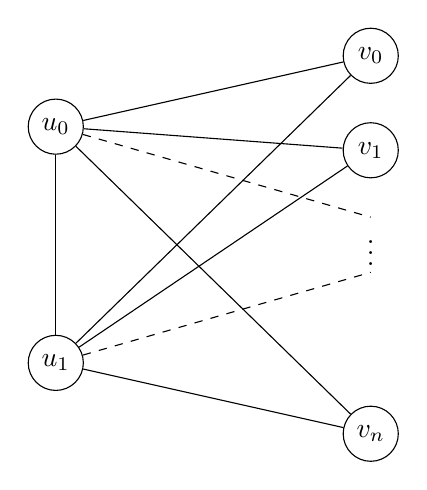
\begin{tikzpicture}[
    vertex/.style={circle, draw, minimum size=7mm, inner sep=0pt},
    every edge/.style={draw}
]

% u vertices
\node[vertex] (u0) at (0, 1.5) {$u_0$};
\node[vertex] (u1) at (0,-1.5) {$u_1$};

% v vertices
\node[vertex] (v0) at (4, 2.4) {$v_0$};
\node[vertex] (v1) at (4, 1.2) {$v_1$};
\node          at (4, 0)       {$\vdots$};
\node[vertex] (vn) at (4,-2.4) {$v_n$};

% Edge between u_0 and u_1
\draw (u0) -- (u1);

% Edges to v_0
\draw (u0) -- (v0);
\draw (u1) -- (v0);

% Edges to v_1
\draw (u0) -- (v1);
\draw (u1) -- (v1);

% Indicate the repeated pattern
\draw[dashed] (u0) -- (4,0.35);
\draw[dashed] (u1) -- (4,-0.35);

% Edges to v_n
\draw (u0) -- (vn);
\draw (u1) -- (vn);

\end{tikzpicture}

Worst case scenario $(u_0, u_1)$ is never removed, resulting $n$ edges removed instead of 1.

\subsubsection*{Simple greedy solution gives 3-approx}
Similar to vertex cover, here we are looking for "triangle cover". Similar to a miximal matching set, we can 
find a maximal set of edge-disjoint triangles. 

\begin{algorithm}[H]
\KwIn{$G=(V,E)$}
\KwOut{Set $R$ of edges to remove}

$R \gets \emptyset$\;

\While{$G$ contains a triangle}{
    Find any triangle $(u,v,w)$ in $G$\;

    $R \gets R \cup \{(u,v),(v,w),(u,w)\}$\;

    Remove edges $(u,v)$, $(v,w)$, and $(u,w)$ from $G$\;
}

\Return{$R$}\;
\end{algorithm}
\begin{proof}
  \subsubsection*{Feasibility}
  Trivial
  \subsubsection*{Guarantee}
  In the optimal solution, every disjoint triangle needs to have at least 1 edge removed in $OPT$, suppose there
  are $k$ disjoint triangles, 
  \[k \leq OPT\]
  Our algorithm remove all edges of all disjoint triangles, 
  \[ALG = 3k \leq 3\cdot OPT\]
\end{proof}
\subsubsection*{Patching with heurstic function of each edge}
Rank all candidate edges by the number of traiangles that can be removed. This can be done in 
polynomial time: 
\begin{algorithm}[H]
\KwIn{$G = (V, E)$}
\KwOut{Number of edges removed $n$}
$H \gets \emptyset$\;
$\text{triangleCount} \gets \emptyset$\; % store edges with associated triangle counts in a tree map
\ForEach{$e = (u, v) \in E$}{
  $H[u] \gets H[u].\text{append}(v)$\;
  $H[v] \gets H[v].\text{append}(u)$\; % add edge information to a hashtable
}   
while any edge has triangle count > 0:
  access the edge with most triangles, 
  remove, 
  update, 
  n++
\Return{$n$\;}
  
\end{algorithm}


\subsection{Fully polynomial-time approximation scheme}
Some pseudo polynomial dynamic programming algorithm can be converted to fully polynomial time approximation algorithm
by sacrificing some precision to make pseudo polynomial term polynomial to the problem size. 

\subsubsection{Woeginger FPTAS}
Given an algorithm in the form of

\begin{algorithm}[H]
\KwIn{vectors $x_1, x_2, \dots, x_n$, where each vector is made of non negative integers not bounded by $n$}
\end{algorithm}


\begin{itemize}
  \item $\epsilon :=$ the required approximation ratio
  \item $G$: there exists an integer $G \geq 0$
  \item $1 + \frac{\epsilon}{2Gn}$
\end{itemize}


\subsubsection*{Example: Knapsack}
First we need to derive 
given the pseudo polynomial dynamic programming solution that runs in $O(nW)$, we can reduce the number of columns 
in the DP table, by reducing the resolution. Given an $\epsilon > 0$, max price of any single item $v_{\max}$, define:
\begin{itemize}
  \item $K = \frac{\epsilon v_{\max}}{n}$
  \item For each item $x_i$, define $v'_i = \lfloor \frac{v_i}{K} \rfloor.$ 
\end{itemize}
We are defining a rounding down function that convert unbounded variable $v_i$ into $v'_i$ that is bounded by an order of $n$: 
\[f: v_i \mapsto \lfloor \frac{n v_i}{\epsilon v_{\max}}\rfloor \]
\[v'_i \leq \frac{n}{\epsilon}\]
The range of total value becomes 
\[R: [0, n v_{\max}] \mapsto [0, n \times \lfloor \frac{n }{\epsilon}\rfloor]\]
Where $\epsilon$ is the parameterized approximation factor, and $v_{\max}$ is constant.
We can transform the original bound $
 O(n^2 W) = O(n^2 v_{\max})$ to $O(n^2 \lfloor \frac{n}{\epsilon}\rfloor)$

First we make the claim that this approximation scheme is feasible (correctness proof)
\[ALG \geq (1 - \epsilon) \cdot OPT\]
\begin{proof}
  Let $\mathcal{O}$ be the optimal choice set, for any item $i$, we are rounding down the value, meaning 
  \[\forall i \in \mathcal{O}, v_i \leq \frac{n}{\epsilon}\]
  \[\sum_{i\in \mathcal{O}} v_i - K \times \sum_{i \in \mathcal{O}} v'_i \leq nK\]

\end{proof}

\subsection{Randomized approximation algorithm}
\subsection{Example: (Minimum) Vertex Cover}
\subsubsection{Greedy approach}
Edge-based greedy selection yields us 2-approximation. 

\begin{algorithm}[H]
  \KwIn{$G = (V, E)$}
  \KwOut{$V' \subseteq V$}
  $V' \gets \emptyset$\;
  \ForEach{$e = (u, v)\in E$}{
    \If{$u \in V'$ or $v \in V'$}{
      continue\;
    }
    \Else {
      $b \gets \text{Random}(0, 1)$\;
      $z \gets \emptyset$\;
      \If{$b = 0$}{
        $z \gets u$\;
      }
      \Else {
        $z \gets v$\;
      }
      $V' \gets V' \cup \{z\}$\;
      $V \gets V \setminus \{z\}$\;
      \ForEach{$e' = (u', v') \in E$}{
        \If {$z = u'$ or $z = v'$}{
          $E \gets E \setminus \{e'\}$\;
        }
      }
    }
  }
  \Return{$V'$}\;
\end{algorithm}
\begin{proof}
  Consider the optimal (minimum) vertex cover $V_{OPT} \subseteq V$, and the greedily chosen $V_{ALG}$. Since our
  algorithm guarantees that 
  \[\forall e = (u, v) \in E, u \in V_{ALG} \lor v \in V_{ALG}\]
  The same applies to the optimal cover, i.e. 
  \[\forall e = (u, v) \in E, u \in V_{OPT} \lor v \in V_{OPT}\]
  Therefore we have $\forall e = (u, v) \in E, $
  WLOG, let $|ALG| > |OPT|$
  Let $A$ and $B$ denotes the set of vertices optimially and not optimally picked, 
  \[A = ALG \cap OPT, \quad B = ALG \setminus OPT\]
  Defined random indicator variable $X_{e = (u, v)}$ such that 
  \[X_{e = (u, v)} = \begin{cases}
    1, \quad u \text{ or } v \in OPT \\
    0, \quad u \text{ or } v \notin OPT 
  \end{cases}\]
  After running hthe algorihtm, all edegs are considered. 
  \[ \mathbb{E}[|A|]= \mathbb{E}[\sum_{e \in E} X_{e = (u)}]\]
  By linear expectation 
  \[\mathbb{E}[|A|] = \sum_{e \in E} \mathbb{E}[X_{e = (u, v)}]\]
\end{proof}



\subsubsection*{Example: Max Cut}
\begin{algorithm}[H]
  
\end{algorithm}

\subsection{Example: weighted MAX-SAT}
Similarly to vertex cover, a simple random assignment gives us 2-approximation. Given a CNF formula
\[\varphi = \bigwedge_{i = 1}^{n} \bigvee_{j \in [1, m]} l_{j}\]
with $n$ clauses, and $m$ boolean variables, a random assignment assigns each variable True or False.

\begin{algorithm}[H]
\KwIn{CNF $\varphi$}
\KwOut{Assignment $A \in \{0, 1\}^m$}
$A \gets \emptyset$\;
\ForEach{$v \in \varphi.V$}{
  $b \gets \text{Random}(0,1)$\;
  $A[v] = b$\;
}
\Return {
  $A$\;
}
\end{algorithm}
\begin{proof}
Define independent probability vatiabble $x_i$ for each variable in $\varphi$. And indicator $\tau(C_i)$ for each clause in $\varphi$, such that 
\[\tau(C_i) = \begin{cases}
  1, \quad C_i \text{is satisfied};\\
  0, \quad \text{otherwise}
\end{cases}\]
Denote the weight of each clause as $w_i$, our objective is to find $\tau$ to maximize
\[\text{weight}(\tau) = \sum_{i}w_i \tau(C_i)\]
\subsubsection*{Unbiased coin: $P(x_i) = \frac{1}{2}$}
The probability of clause $C_i$ 
evaluates to true can be expressed as 
\[P(C_i) = 1 - (\frac{1}{2})^{|C_i|}\]
We can express the expectation 
\[\mathbb{E}[\text{weight}(\tau)] = \sum_{i} w_i (1 - \frac{1}{2^{|C_i|}}) \geq \frac{1}{2}\sum_i w_i\]
We know that the optimal is at most the sum of weights of all clauses (when all clasues are satisfied), we have
\[\mathbb{E}[\text{weight}(\tau)] \geq \frac{1}{2}\sum_i w_i \geq \frac{1}{2}\cdot OPT\]


\subsubsection*{Biased coin}
Suppose the coin flip is biased, with a probabiluty of $p$ instead of $\frac{1}{2}$. Let $\ell^+_i$ denote the number of positive literals in clause $C_i$, and $\ell_i^-$ for negative literals. We can similarly express the probability of one clause the evaluates to true as
\[P(C_i) = 1 - (p)^{\ell^-_i}(1 - p)^{\ell^+_i}\]
WLOG, let $p \geq \frac{1}{2}$, we have 
\[P(C_i) = 1 - p^{\ell^-_i}(1 - p)^{\ell^+_i} \geq 1 - p^{\ell^-_i}\cdot p^{\ell^+_i} = 1 - p^{|C_i|}\]
Then we can express the expectation of total weight as
\[\mathbb{E}[\text{weight}(\tau)] = \sum_i w_i [1 - p^{\ell^-_i}(1 - p)^{\ell^+_i}] \geq \sum_i w_i (1 - p^{|C_i|})\]


Similar to the unbiased case, we need to construct a lower bound on the probability of each clasue to evaluate to true. 
In the uniased casse, we have $P[C_i] = \frac{1}{2}$ for $|C_i| = 1$, regardless if the singleton clause contains a positive or negative literal. 
And $\forall |C_j| > |C_i| > 1, (1 - (\frac{1}{2})^|C_i|) < (1 - (\frac{1}{2})^|C_j|)$, which means the probability is monotonously decreasing as the 
length of the clause. 

This is not the case for a biased coin, as we have $p > \frac{1}{2}$, therefore we cannot effectively bound the probaility of a clause is satisfiable. 
For now we patch this by making the following assumption: all singleton contains only positive literals. Now we can construct a non-trivial lower bound 
\[q = \min(p, 1 - p^2)\]
Where $p$ represents the case of singleton clauses, and $1 - p^2$ take accont of clause of size $\geq 2$, as the 
monontoncity still holds here. It follows 
\[\mathbb{E}[\text{weight}(\tau)] \geq \min(p, 1 - p^2) \sum_i w_i \geq \min(p, 1 - p^2)\cdot OPT\]
Now we have expressed the approximation factor in one variable $p$, finding the maximun we have 
\[\mathbb{E}[\text{weight}(\tau)] \geq \min(p, 1 - p^2)\cdot OPT \approx \frac{\sqrt{5} - 1}{2} \cdot OPT\]
\end{proof}



\subsection{LP relaxation}
Similar to propositional logics, we can use integer linear system to model decision and choice based optimization problem.
Integer linear programming is NP-hard, but LP in real is not. We may relax a ILP formulation to LP, and round the solutions to 
integer in a way that the feasibility is preserved. 
\begin{enumerate}
  \item Model problem as an instance of ILP
  \item Replace $x_i \in \{0, 1\} $ to $x^*_i \in [0,1]$, relax to LP
  \item solve
  \item Rounding 
\end{enumerate}
\subsubsection*{Example: weighted MAX-SAT}
Consider the assignment of each individual variable $v_i$ as a binray variable $x_i$, and the truth value of each clauuse $C_j$ using a 
binary variable $y_i$ dependent on the assignmentd. 
\begin{itemize}
  \item Constraints: $\forall C_i$
  \[
    \sum_{v_j \in C_i} x_j + \sum_{\neg v_k \in C_i} (1 - x_k) \geq y_i
  \]
  \item Goal: maximize
\end{itemize}
Note here we dont need additional clauses to enforce structural constraints like in PL. (may not be the case for other problems, see MAX-DICUT)
\subsubsection*{Use real solution as expectation to assign integral values}
after solving, $\forall x_i$, we assign variable $v_i$ to be true at probability of $x_i^*$
\[Pr(v_i) = x_i\]
We can express the probabality of clause $C_i$ to be true as 
\[Pr(C_i) = 1 - \prod_{v_j \in C_i} (1 - x_j^*) \cdot \prod_{\neg v_k^* \in C_i} x_k^*\]
thus 
\[\mathbb{E}[\tau(C_i)] = 1 - \prod_{v_j \in C_i} (1 - x_j^*) \cdot \prod_{\neg v_k^* \in C_i} x^*_k\]
\[\sum_{C_i \in \varphi} w_i \cdot \mathbb{E}[\tau(C_i)], \quad\quad OPT = \sum_{C_i \in \varphi} w_i \cdot y_i^*\]
\subsubsection*{Bound Analysis}
From our LP formulation 
\[y_i^* \leq \sum_{v_j \in C_i} x_j^* + \sum_{v_k \in C_i} (1 - x_k^*)\]
\[\mathbb{E}[\tau(C_i)] = 1 - \prod_{v_j \in C_i} (1 - x_j^*) \cdot \prod_{\neg v_k^* \in C_i} x^*_k\]
Using AM-GM inequality: 
\[(\prod_{i=1}^k a^i)^{\frac{1}{k}} \leq \frac{1}{k} \sum_{i=1}^{k}a_i, \quad\quad \prod_{i=1}^{k} a_i \leq (\frac{1}{k} \sum_{i=1}^k a_i)^k\]
Use inequality
\[\mathbb{E}[\tau(C_i)] \geq 1 - \left[ \frac{1}{|C_i|} \left(\sum_{v_j \in C_i} (1 - x_j^*) + \sum_{\neg v_k \in C_i} x_k^* \right)\right]^{\frac{1}{|C_i|}}\]
\[= 1 - \left[ 1 - \frac{1}{|C_i|} \left( \sum_{v_j \in C_i} x_j^* + \sum_{\neg v_k \in C_i} (1 - x_k^*) \right)\right]^{\frac{1}{|C_i|}}\]
\[\geq 1 - \left[ 1 - \frac{1}{|C_i|} y^*_i\right]^{\frac{1}{|C_i|}}\]
From standard inequalities 
\[1 - x \leq e^{-x}, \quad\quad 1 + x \leq e^x\]
\subsection{Inapproximability}









\section{Linear programming and integer programming}
\subsection{ILP formulation from finite space FOL}
\begin{enumerate}
  \item Express logical constraints using FOL formula
  \item Convert FOL formula to grounded propositional logic formula
  \item Binary encoding
\end{enumerate}
\begin{table}[H]
\centering

\begin{tabular}{l l}
\hline
\textbf{Boolean Expression} & \textbf{Linear Constraint} \\
\hline

$\displaystyle \bigvee_{i\in I} A_i$
&
$\displaystyle \sum_{i\in I} A_i \ge 1$
\\[6pt]

$\displaystyle \bigwedge_{i\in I} A_i$
&
$\displaystyle \sum_{i\in I} A_i = |I|$
\\[6pt]

$\displaystyle \neg\left(\bigvee_{i\in I} A_i\right)$
&
$\displaystyle \sum_{i\in I} A_i = 0$
\\[6pt]

$\displaystyle \neg\left(\bigwedge_{i\in I} A_i\right)$
&
$\displaystyle \sum_{i\in I} A_i \le |I|-1$
\\[6pt]

$\displaystyle
\left(\bigvee_{i\in I} A_i\right)\rightarrow B$
&
$\displaystyle
|I|B-\sum_{i\in I}A_i \ge 0$
\\[6pt]

$\displaystyle
\left(\bigwedge_{i\in I} A_i\right)\rightarrow B$
&
$\displaystyle
B-\sum_{i\in I}A_i \ge -( |I|-1)$
\\[6pt]

$\displaystyle
A\rightarrow\left(\bigvee_{i\in I}B_i\right)$
&
$\displaystyle
\sum_{i\in I}B_i-A\ge0$
\\[6pt]

$\displaystyle
A\rightarrow\left(\bigwedge_{i\in I}B_i\right)$
&
$\displaystyle
\sum_{i\in I}B_i-|I|A\ge0$
\\

\hline
\end{tabular}

\caption{Generalized Boolean expressions using binary variables.}
\end{table}
\subsubsection*{Example: Vertex cover}
Express the constraints in FOL is simple, define relation $S(v)$ as $v \in VC$
\[\forall (u, v) \in E, S(u) \lor S(v)\]
Define selection indicator variable $x_v$
\[x_v = \begin{cases}
  1, \quad \text{ S(v)}\\
  0, \quad \text{ otherwise}
\end{cases}\]
Use the encoding, we have 
\[\forall (u, v ) \in E, \quad x_u + x_v \geq 1\]
The goal becomes to find 
\[\min(\sum_{v \in V} x_v )\]
\subsection{Encoding decision variables and facts}
\subsubsection*{Se cover}
given a set of elements $U = \{u_1, u_2, \dots, u_n\}$, and a set of sets $\mathcal{S} = \{S_1, S_2, \dots, S_m\}$, assuming 
$\bigcup_{S\in \mathcal{S}} = U$, find a set cover to minimize
\[\sum_{S \in S' \subseteq \mathcal{S}'} w_S\]
\subsubsection*{Decision variable}
We will need to use a decision variable to encode 
\begin{itemize}
  \item the coverage of an element: $x_i$
  \item the choice of sets: $y_j$
\end{itemize}
Define unary relation $S(u_i)$ to denote that $u_i$ is covered, and $R(S_j)$ as set $S_j$ is chosen 
\[x_i = \begin{cases}
  1, S(u_i)\\
  0, \text{ otherwise}
\end{cases}
\qquad
y_j = \begin{cases}
    1, R(S_j)\\
    0, \text{ otherwise}
  \end{cases}\]
Beside we can also define more relations to describe the structures, for example 
$T(u_i, S_j)$ to represent $u_i \in S_j$. Then we can express the constriants as 
\[\forall u_i (\exists S_j (T(u_i, S_j) \land R(S_j)))\]
\subsection{Randomized Rounding}
To map LP result in $[0, 1]$ back to $\{0, 1\}$ rounding is needed. The most naive rounding scheme would be
to assign $x$ with 1 at probability of $x^*$
\[\mathbb{E}[x = 1] = x^*\]
\subsubsection*{Example: MAX-SAT}
see above 
\subsubsection*{Example: MAX-DICUT}
Sometimes directly using $x$ may not be optimal. For example MAX-DICUT

\subsubsection*{Let $p_i = \frac{1}{4} + \frac{x_i}{2}$}
Recall the LP formulation, the relaxed formulation reuslt is 
\[LP^* = \sum_{(i, j) \in A} w_{ij}z_{ij}\]
The probability of an edge being admitted to the dicut is 
\begin{align*}
P[(i \in U) \land j \in W] &= p_i \cdot (1 - p_j)  \\
&= (\frac{1}{4} + \frac{x_i}{2})(1 - \frac{1}{4} - \frac{x_j}{2})\\
&= (\frac{1}{4} + \frac{x_i}{2})(\frac{1}{4} + \frac{1 - x_j}{2}) 
\end{align*}
From the constraints, which are 
\begin{align*}
  z_{ij} \leq x_i\\
  z_{ij} \leq 1 - x_j
\end{align*}
We have 
\[\frac{1}{4} + \frac{x_i}{2} \geq \frac{1}{4} + \frac{z_{ij}}{2}, \quad\quad \frac{1}{4} + \frac{1-x_j}{2} \geq \frac{1}{4} + \frac{z_{ij}}{2} \]
therefore 
\begin{align*}
P[(i \in U) \land j \in W] &\geq \left(\frac{1}{4} + \frac{z_{ij}}{2} \right)^2  \\
&=\frac{z_{ij}}{2} + \frac{(2z_{ij} -1)^2}{16}\\
&\geq \frac{z_{ij}}{2}
\end{align*}
Define indicator variable $X_{ij}$ to indicate $arc(i, j)$ is in dicut
\begin{align*}
  \mathbb{E}[\text{weight}(A)] &= \sum_{(i, j) \in A} w_{ij} \mathbb{E}[X_{ij}]\\
  &= \sum_{(i,j) \in A} w_{ij} P[(i \in U) \land (j \in W)]\\
  &\geq \frac{1}{2} \sum_{(i,j) \in A} w_{ij} z_{ij}\\
  & = \frac{1}{2} LP^* \geq \frac{1}{2} \cdot OPT
\end{align*}



\subsubsection*{Native probability assignemnt}
We will see now using $p_i = x_i$ will not give as good approximation. 
\begin{align*}
  P[(i \in U) \land j \in W] &= p_i \cdot (1 - p_j) \\
  &= x_i \cdot (1 - x_j)\\
  &\geq z_{ij}^2
\end{align*}
thus 
\begin{align*}
  \mathbb{E}[\text{value}(A)]&=\sum_{(i,j)\in A} w_{ij} \mathbb{E}[X_{ij}]\\
  &\geq \sum_{(i,j)\in E} w_{ij} z_{ij}^2
\end{align*}
using Cauchy-scharwz inequality: 
\[(\sum_{i=1}^{n} a_i b_i)^2 \leq (\sum_{i=1}^{n} a_i^2)(\sum_{i=1}^{n} b_i^2)\]
rearrange by letting $a_{ij} = \sqrt{w_{ij}} z_{ij}, b_{ij} = \sqrt{w_{ij}}$
\begin{align*}
  (\sum_{(i,j)\in E} w_{ij} z_{ij})^2 &\leq (\sum_{(i,j)\in E} w_{ij})(\sum_{(i,j)\in E} w_{ij} z_{ij}^2)\\
  (\sum_{(i,j)\in E} w_{ij} z_{ij}^2) &\geq \frac{(\sum_{(i,j)\in E} w_{ij} z_{ij})^2}{\sum_{(i,j)\in E} w_{ij}}\\
  &= \frac{(LP^*)^2}{\sum_{(i,j)\in E} w_{ij}}
\end{align*}
Let 
\[L = LP^*, \quad\quad W = \sum_{(i,j)\in E} w_{ij}\]
\begin{align*}
  \mathbb{E}[ALG] \geq \frac{L^2}{W} &= \alpha L\\
  \alpha &= \frac{L}{W}
\end{align*}
\subsubsection*{Fidning optimal linear expression of $p$ in $x$}
Let the probability of assignment $p$ be 
\[p_i = a + bx_i\]
Using the same relaxation result, the probability of an edge to be admitted is 
From $z_{ij} \leq x_i$ and $z_{ij} \leq 1-x_j$, we have
\begin{align*}
P[(i \in U) \land (j \in W)]
&= p_i(1-p_j)\\
&= (a+bx_i)(1-a-bx_j)\\
&= (a+bx_i)\bigl((1-a-b)+b(1-x_j)\bigr)\\
&\geq (a+bz_{ij})(1-a-b+bz_{ij}).
\end{align*}
To force a square term, let $c = 1 - a - b$, such that 
\begin{align*}
P[(i \in U) \land (j \in W)] &\geq (a + bz_{ij})(c + bz_{ij})  \\
&= ac + b(a+c)z_{ij} + b^2 z_{ij}^2\\
&= ac + b(1-b)z_{ij} + b^2 z_{ij}^2\\
\end{align*}
Since how the value of $1-b$ splits betweeen $a$ and $c$ now only depends on $ac$, and we have
\[ac \leq \left(\frac{a + c}{2}\right)^2\]
We want to maximize $ac$, as the difference square term will minus some factor of $z_{ij}$ term: $\gamma \cdot z_{ij}$, and the remaining $z_{ij}$ term will be
$[b (1 - b) + \gamma ] z_{ij} = \alpha z_{ij}$, where $\alpha$ is the approximation factor which we want to minimize. According to the 
inequality, $ac$ is maximized when we have 
\[a=c \implies a = 1 - a - b, \qquad a = \frac{1-b}{2}\] 
Then we subsetitute $c$, the original probability bound gives us
\begin{align*}
P[(i\in U)\land(j\in W)]
&\geq (a+bz_{ij})^2\\
&= 4abz_{ij} + (a-bz_{ij})^2\\
&\geq 4abz_{ij}\\
\alpha &= 4ab
\end{align*}
Substitute $a$ with $b$, 
\begin{align*}
  \alpha &= 4ab\\
  &= 2b(1-b)\\
  &= -2(b^2 - b + \frac{1}{4}) + \frac{1}{2}\\
  &\geq \frac{1}{2}
\end{align*}








\section{Network flow}
\subsection{Integer Network flow}
\subsubsection{Ford--Fulkerson Algorithm}
Constraints:
\begin{itemize}
  \item Capacity constraint: 
  \[\forall (u, v) \in E, f(u, v) \leq c(u, v)\]
  \item Conservation constraint:
  \[\forall v \in V \setminus \{s, t\}, \sum_{(u, v) \in E} f(u, v) = \sum_{(v, z) \in E} f(v, z)\]
  \item Goal: maximize $value(f)$, flow leaving $s$:
  \[\sum_{(s, v) \in E} f(s, v)\]
\end{itemize}

\begin{algorithm}[H]
  \KwIn{Flow network $G=(V,E)$, capacities $c:E\to\mathbb{Z}_{\ge 0}$,
        source $s$, sink $t$}
  \KwOut{Maximum flow $f$}

  \ForEach{$e\in E$}{
    $f(e)\gets 0$\;
  }

  Construct residual graph $G_f$\;

  \While{$\exists s$--$t$ path $P$ in $G_f$}{
    
    Choose any $s$--$t$ path $P$ in $G_f$\;

    $\Delta \gets \displaystyle\min_{(u,v)\in P} c_f(u,v)$\;

    \ForEach{$(u,v)\in P$}{
      \eIf{$(u,v)\in E$}{
        $f(u,v)\gets f(u,v)+\Delta$\;
      }{
        $f(v,u)\gets f(v,u)-\Delta$\;
      }
    }

    Update residual graph $G_f$\;
  }

  \Return $f$\;
\end{algorithm}
\paragraph{Explanation.}
Ford--Fulkerson starts with the zero flow and repeatedly searches for an
arbitrary augmenting path from the source $s$ to the sink $t$ in the
residual graph $G_f$.

For a current flow $f$, the residual capacity is defined by
\[
c_f(u,v)=
\begin{cases}
c(u,v)-f(u,v), & (u,v)\in E,\\[2mm]
f(v,u), & (v,u)\in E,\\[2mm]
0, & \text{otherwise}.
\end{cases}
\]

Hence, the residual graph is
\[
G_f=(V,E_f),
\qquad
E_f=\{(u,v)\mid c_f(u,v)>0\}.
\]

If an $s$--$t$ augmenting path $P$ exists, let
\[
\Delta
=
\min_{(u,v)\in P} c_f(u,v)
\]
be the bottleneck residual capacity of the path.

The flow is augmented by $\Delta$ along $P$. For a forward edge
$(u,v)\in E$, we increase the flow:
\[
f(u,v)\gets f(u,v)+\Delta.
\]

For a backward residual edge $(u,v)$ corresponding to an original edge
$(v,u)\in E$, we decrease the original flow:
\[
f(v,u)\gets f(v,u)-\Delta.
\]

After each augmentation, the residual graph is updated. The algorithm
terminates when no $s$--$t$ path exists in the residual graph. By the
Max-Flow Min-Cut Theorem, the resulting flow is a maximum flow.

For integer capacities, every residual capacity and every bottleneck
value $\Delta$ is integral. Therefore, each augmentation increases the
flow value by at least $1$. Hence Ford--Fulkerson performs at most
$|f^*|$ augmentations, where $|f^*|$ is the value of a maximum flow.

If finding an arbitrary augmenting path and updating the flow takes
$O(|E|)$ time, the total running time is
\[
O(|E|\cdot |f^*|).
\]

Thus, Ford--Fulkerson is pseudo-polynomial for integer capacities, since
$|f^*|$ may be exponentially large in the number of bits required to
encode the capacities.

\subsection{$s-t$ cut}
Given $G = (V, E)$ and $s, t \in {V}$ a s-t cut is defined as 
\[\{(u, v)\mid u \in A, v \in bar{A}\}\]
where 
\[A \subseteq V, s\in A, t \in \bar{A} \]

\subsubsection*{Capacity of a cut}
Define the capacity of the cut as the sum of the capacity of edges
\[c(A, \bar{A}) = \sum_{(u, v) \in E, u \in A, v \in \bar{A}} c(u, v)\]
\subsubsection*{Generalized conservation constraint}
Consider any $s-t$ cut, $\forall v\in V$ 
\[f_{out}(v) - f_{in}(v) = \begin{cases}
    0, u \in V \setminus \{s, t\}\\
    value(f), u = s\\
    -value(f), u = t
\end{cases}\]
Using the constraint we can define the in/outflow of $A$ in a $s-t$ cut:
\begin{align*}
  f_{out}(A) &= \sum_{(u, v) \in E, u \in A, v \in \bar{A}} f(u, v)\\
  f_{in}(A) &= \sum_{(v, u) \in E, u \in A, v \in \bar{A}} f(u, v)
\end{align*}
\begin{lemma}
  \[f_{out}(A) - f_{in}(A) = value(f)\]
\end{lemma}
\begin{proof}
  \begin{align*}
    f_{out}(A) - f_{in}(A)&= \sum_{u \in A} \sum_{(u, x) \in E} f(u, x) - \sum_{u \in A} \sum_{(x, u)\in E} f(x, u)\\
    &=\sum_{u\in A}\left( \sum_{(u, x) \in E} f(u, x) - \sum_{(x, u) \in E} f(x, u)\right)\\
    &= \sum_{u\in A} \left( f_{out}(u) - f_{in}(u) \right)\\
    s\in A \implies \\
    \sum_{u\in A} \left( f_{out}(u) - f_{in}(u) \right) &= \sum_{u \in A \setminus \{s\}} 0 + (f_{out}(s) - f_{in}(s))\\
    &= value(f)
  \end{align*}
\end{proof}
\begin{corollary}
  $f_{out}(A) - f_{in}(A) \leq c(A, \bar{A})$
\end{corollary}
\subsection{Max-flow and min-cut}
\subsubsection*{Max-flow $\leq$ min-cut}
We will be proving an equall strong statement: any valid flow $\leq$ any valid cut
\begin{proof}
  Consider any arbitrary cut, $(A, \bar{A})$, 
  from lemma 3.1, we have 
  \begin{align*}
  value(f) &= f_{out}(A) - f_{in}(A)\\    
  &\leq f_{out}(f)\\
  &= \sum_{(u,v) \in E, u \in A, v\in \bar{A}} f(u, v)\\
  &\leq \sum_{(u,v) \in E, u \in A, v\in \bar{A}} c(u, v)
  \end{align*}
  Since the partition is arbitrary, any flow through is upper bounded by any cut.
\end{proof}
\subsubsection*{Max-flow $\geq$ min-cut}
Here we will prove that upon FF termination, for partiton $s \in S, t \in T$ 
\[c(S, T) = value(f)\]
\begin{proof}
Using the FF algorithm, at termination stage, the residual graph has no path from $s$ to $t$.     
Suppose otherwise, 
\subsubsection*{If $\exists (u, v)\in E, u\in S, v\in T, f(u, v) < c(u, v)$}
Not all edges from $S$ to $T$ are saturated in $G$, meaning exists residual edges will appear in $G_f$, contradiction to the termination condition.
And by capacity constraint, 
\[\forall u \in S, v\in T, f(u, v) = c(u, v)\]
Similarly, we can show that 
\[\forall u \in S, v\in T, f(v, u) = 0\]
As otherwise, there exist such a residual edge $(u, v)$ in $G_f$, $t$ becomes reachable from $s$, contradicting to the termination condition.
\begin{align*}
  value(f) &= \sum_{(u,v) \in E, u \in S, v\in T} f(u, v) - \sum_{(v, u) \in E, u \in S, v\in T} f(v, u)\\
  &= \sum_{(u,v) \in E, u \in S, v\in T} c(u, v) - 0\\
  &= c(S, T)
\end{align*}
Since upon termination of FF, a valid flow that has the same value as a valid cut are produced, we have 
\[\text{min-cut} \leq c(S, T) = value(f) \leq \text{max-flow}\]
\end{proof}

\subsection{Pathological example of naive FF}
FF may not terminate when edge capacity are real, when a particular pathological path choices are made. Consider the following graph:
\usetikzlibrary{arrows.meta,positioning}

\begin{figure}[H]
\centering

\begin{tikzpicture}[
    >=Stealth,
    vertex/.style={
        circle,
        draw,
        minimum size=8mm,
        inner sep=0pt
    },
    edge/.style={->, thick},
    special/.style={->, very thick}
]

% ------------------------------------------------
% Vertices
% Mapping from top to bottom:
% v4, v3, v2, v1

\node[vertex] (s)  at (-3,0)   {$s$};

\node[vertex] (v4) at (0, 2.4) {$v_4$};
\node[vertex] (v3) at (0, 0.8) {$v_3$};
\node[vertex] (v2) at (0,-0.8) {$v_2$};
\node[vertex] (v1) at (0,-2.4) {$v_1$};

\node[vertex] (t)  at (3,0)    {$t$};

% ------------------------------------------------
% Large-capacity edges

\draw[edge]
    (s) -- node[above left] {$M$} (v4);

\draw[edge]
    (s) -- node[above] {$M$} (v2);

\draw[edge]
    (s) -- node[below left] {$M$} (v1);

\draw[edge]
    (v4) -- node[above right] {$M$} (t);

\draw[edge]
    (v3) -- node[above] {$M$} (t);

\draw[edge]
    (v1) -- node[below right] {$M$} (t);

% ------------------------------------------------
% Special edges

% e2 : v4 -> v3, capacity r
\draw[special]
    (v4) -- node[right] {$e_2:r$} (v3);

% e3 : v2 -> v3, capacity 1
\draw[special]
    (v2) -- node[right] {$e_3:1$} (v3);

% e1 : v2 -> v1, capacity 1
\draw[special]
    (v2) -- node[right] {$e_1:1$} (v1);

\end{tikzpicture}
\end{figure}

\paragraph{Pathological augmenting-path sequence.}

First choose the initial augmenting path
\[
P_0=(s,v_2,v_3,t),
\]
which sends one unit of flow and saturates $e_3$.

Define the following residual augmenting paths:
\begin{align*}
P_1 &= (s,v_4,v_3,v_2,v_1,t),\\
P_2 &= (s,v_2,v_3,v_4,t),\\
P_3 &= (s,v_1,v_2,v_3,t).
\end{align*}

Notice that some edges in these paths are
\emph{reverse residual edges} rather than original edges of $G$.
In particular,
\begin{align*}
P_1 &: \quad v_3 \to v_2
      \text{ is the reverse residual edge of }e_3,\\
P_2 &: \quad v_3 \to v_4
      \text{ is the reverse residual edge of }e_2,\\
P_3 &: \quad v_1 \to v_2
      \text{ is the reverse residual edge of }e_1.
\end{align*}

After $P_0$, repeatedly choose
\[
\boxed{
P_1,\;P_2,\;P_1,\;P_3
}
\]
indefinitely. Thus the complete sequence is
\[
\boxed{
P_0,\;
(P_1,P_2,P_1,P_3),\;
(P_1,P_2,P_1,P_3),\;
(P_1,P_2,P_1,P_3),\ldots
}
\]

If the residual capacities of $(e_1,e_2,e_3)$ are initially
\[
(a_n,a_{n+1},0),
\]
then one four-path cycle gives
\begin{align*}
(a_n,a_{n+1},0)
&\xrightarrow{P_1}
(a_{n+2},0,a_{n+1})\\
&\xrightarrow{P_2}
(a_{n+2},a_{n+1},0)\\
&\xrightarrow{P_1}
(0,a_{n+3},a_{n+2})\\
&\xrightarrow{P_3}
(a_{n+2},a_{n+3},0).
\end{align*}

Here
\[
a_{n+2}=a_n-a_{n+1},
\qquad
a_0=1,
\qquad
a_1=r.
\]

Since
\[
r^2=1-r,
\]
we have
\[
a_n=r^n>0
\]
for every finite $n$. Therefore every cycle leaves another
positive-capacity augmenting path, so Ford--Fulkerson never terminates.



\begin{lemma}[Integrality of max-flow]
If all edges have integer capacity, there exists a max-flow that is of integer value.
\end{lemma}
\subsection{Edmonds-Karp}
\begin{algorithm}[H]
  \KwIn{Flow network $G=(V,E)$, capacities $c:E\to\mathbb{Z}_{\ge 0}$,
        source $s$, sink $t$}
  \KwOut{Maximum flow $f$}
  $k\gets \max(E)$\;
  \ForEach{$e\in E$}{
    $f(e)\gets 0$\;
  }

  Construct residual graph $G_f$\;
  \While{$k \geq 1$}{

  \While{$\exists s$--$t$ path $P$ in $G_f$, which has capacity $\geq k$}{
    
    Choose any $s$--$t$ path $P$ in $G_f$\;

    $\Delta \gets \displaystyle\min_{(u,v)\in P} c_f(u,v)$\;

    \ForEach{$(u,v)\in P$}{
      \eIf{$(u,v)\in E$}{
        $f(u,v)\gets f(u,v)+\Delta$\;
      }{
        $f(v,u)\gets f(v,u)-\Delta$\;
      }
    }

    Update residual graph $G_f$\;
  }
  $k \gets \frac{k}{2}$
  }

  \Return $f$\;
\end{algorithm}
Upon termination of one inner loop, $\not\exists $ an $s-t$ path that has capacity $\geq k$, meaning a
"cut" formed at this stage, 
\begin{itemize}
  \item $\forall (u, v) \in E, u \in S, v \in T, c(u,v) - f(u, v) < k$
  \item $\forall (v, u) \in E, u \in S, v \in T, f(v, u) < k$
\end{itemize}
Consequently, 
\begin{align*}
value(f) &= f_{out}(S) - f_{in}(S) \\
&= \sum_{(u, v) \in E, u \in S, v \in T} f(u, v) - \sum_{(v, u) \in E, u \in S, v \in T} f(v, u)\\
&>\sum_{(u, v) \in E, u \in S, v \in T} \left(c(u, v) - k\right) - \sum_{(v, u) \in E, u \in S, v \in T} k\\
&> c(S, T) - |E|k\\
&> value(f_{\max}) - |E|k
\end{align*}
At the end of this iteration, $k$ is halved. thus we have 
\[value(f) > value(f_{\max}) - 2k |E|\]
According to the inner loop condition, the path selected has capacity at least $k$, thus the bottleneck capacity
$\Delta \geq k$, each inner loop iteration flow is increased by at least k, thus we need at most $2|E|$ iterations we can reach $f_{\max}$
Therefore the overall complextity is
\[O(|E|^2 \cdot \log_2(c))\]






\subsection{Real capacity network flow}
\subsubsection*{Dinitz}
\begin{algorithm}[H]
  \KwIn{Flow network $G=(V,E)$, capacities $c:E\to\mathbb{Z}_{\ge 0}$,
        source $s$, sink $t$}
  \KwOut{Maximum flow $f$}
  $k\gets \max(E)$\;
  \ForEach{$e\in E$}{
    $f(e)\gets 0$\;
  }

  Construct residual graph $G_f$\;

  \While{Let $P$ be the shortest $s-t$ path in $G_f$}{
    
    Choose any $s$--$t$ path $P$ in $G_f$\;

    $\Delta \gets \displaystyle\min_{(u,v)\in P} c_f(u,v)$\;

    \ForEach{$(u,v)\in P$}{
      \eIf{$(u,v)\in E$}{
        $f(u,v)\gets f(u,v)+\Delta$\;
      }{
        $f(v,u)\gets f(v,u)-\Delta$\;
      }
    }

    Update residual graph $G_f$\;
  }

  \Return $f$\;
\end{algorithm}














\end{document}
